\chapter{上下文管理}

\section{with 简化资源管理}
在 Python 编程中，资源管理是一个重要但容易被忽视的环节。
\codeinline{with} 关键字为我们提供了一种优雅的方式来处理文件操作、数据库连接等需要明确释放资源的场景。

with 是 Python 中的一个关键字，用于上下文管理协议（Context Management Protocol）。它简化了资源管理代码，
特别是那些需要明确释放或清理的资源（如文件、网络连接、数据库连接等）。

\subsection{基本语法}
\begin{lstlisting}[style=demostyle,numbers=none]
'''
expression 返回一个支持上下文管理协议的对象
as variable 是可选的，用于将表达式结果赋值给变量
'''    
with expression [as variable]:
    # 代码块
\end{lstlisting}

\begin{enumerate}[label=\arabic*)]
    \item 文件操作
\begin{lstlisting}[style=pythonstyle]
# 文件操作    
with open('example.txt', 'r') as file:
    content = file.read()
    print(content)
# 文件已自动关闭
\end{lstlisting}

\begin{lstlisting}[style=pythonstyle]
# 同时打开多个文件
with open('input.txt', 'r') as infile, open('output.txt', 'w') as outfile:
    content = infile.read()
    outfile.write(content.upper())
\end{lstlisting}

    \item 数据库连接
\begin{lstlisting}[style=pythonstyle]
import sqlite3

with sqlite3.connect('database.db') as conn:
    cursor = conn.cursor()
    cursor.execute('SELECT * FROM users')
    results = cursor.fetchall()
# 连接自动关闭
\end{lstlisting}

    \item 线程锁

\begin{lstlisting}[style=pythonstyle]
import threading
lock = threading.Lock()
with lock:
    # 临界区代码
    print("这段代码是线程安全的")
\end{lstlisting}

    \item 临时修改系统状态
\begin{lstlisting}[style=pythonstyle]
import decimal
with decimal.localcontext() as ctx:
    ctx.prec = 42  # 临时设置高精度
    # 执行高精度计算
# 精度恢复原设置
\end{lstlisting}
\end{enumerate}



\subsection{工作原理}
with 语句背后是 Python 的上下文管理协议，该协议要求对象实现两个方法：
\begin{enumerate}[label=\arabic*)]
    \item \codeinline{\_\_enter\_\_()}：进入上下文时调用，返回值赋给 as 后的变量。
    \item \codeinline{\_\_exit\_\_()}：在 with 块结束后调用，用于清理资源。
\end{enumerate}
\begin{figure}[htpb]
    \centering
    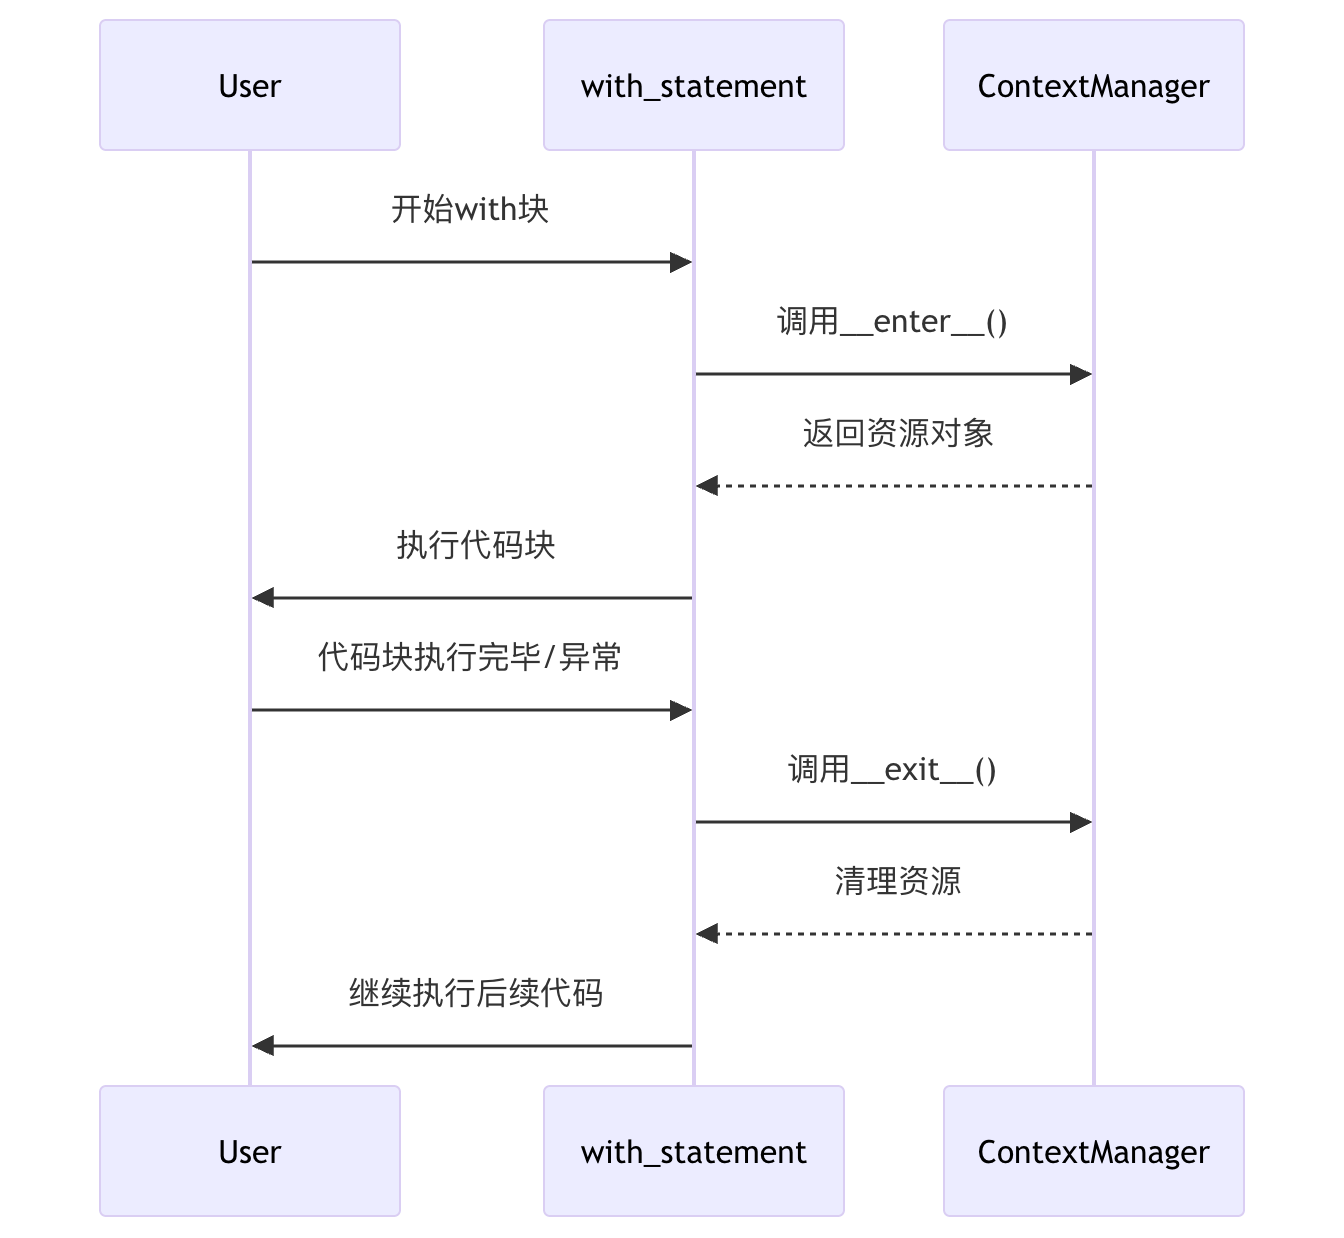
\includegraphics[width=0.6\textwidth]{part/存储/上下文管理/pic/with上下文管理执行流程.png}
    \caption{with 上下文管理执行流程}
\end{figure}


\section{创建自定义的上下文管理器}
\subsection{类的方式}
我们可以通过实现 \codeinline{\_\_enter\_\_()} 和 \codeinline{\_\_exit\_\_()} 方法创建自定义的上下文管理器
\begin{lstlisting}[style=demostyle,numbers=none]
def __enter__(self):
    # 创建资源
    return self
    
'''
exc_type：异常类型
exc_val：异常值
exc_tb：异常追踪信息

如果 __exit__() 返回 True，则表示异常已被处理，不会继续传播；返回 False 或 None，异常会继续向外传播。
'''    
def __exit__(self, exc_type, exc_val, exc_tb):
    # 释放资源
    return False    
\end{lstlisting}

\begin{lstlisting}[style=pythonstyle]
class Timer:
    def __enter__(self):
        import time
        self.start = time.time()
        return self
    
    def __exit__(self, exc_type, exc_val, exc_tb):
        import time
        self.end = time.time()
        print(f"耗时: {self.end - self.start:.2f}秒")
        return False

# 使用示例
with Timer() as t:
    # 执行一些耗时操作
    sum(range(1000000))
\end{lstlisting}

\subsection{contextlib 模块}
\begin{lstlisting}[style=pythonstyle]
from contextlib import contextmanager

@contextmanager
def tag(name):
    print(f"<{name}>")
    yield
    print(f"</{name}>")

# 使用示例
with tag("h1"):
    print("这是一个标题")
\end{lstlisting}    
